\documentclass{article}
\usepackage[margin=1in]{geometry}
\usepackage{amsmath, amssymb, amsthm}
\usepackage{enumitem}

% color!
\usepackage[dvipsnames]{xcolor}
% \definecolor{mypink1}{rgb}{0.858, 0.188, 0.478}
% \definecolor{mypink2}{RGB}{219, 48, 122}
% \definecolor{mypink3}{cmyk}{0, 0.7808, 0.4429, 0.1412}
% \definecolor{mygray}{gray}{0.6}

% colored links
\usepackage{hyperref}
\hypersetup{
    colorlinks=true,
    linkcolor=blue,
    filecolor=magenta,      
    urlcolor=blue,
    }

% Inputting psuedocode
\usepackage{algorithm}
\usepackage[noend]{algpseudocode}
\renewcommand\algorithmicdo{}

% Inputting Python code
\definecolor{textblue}{rgb}{.2,.2,.7}
\definecolor{textred}{rgb}{0.54,0,0}
\definecolor{textgreen}{rgb}{0,0.43,0}
\usepackage{upquote}
\usepackage{listings}
\lstset{
    language=Python, 
    tabsize=4,
    basicstyle={\ttfamily},
    keywordstyle=\color{textblue},
    commentstyle=\color{textgreen},
    stringstyle=\color{textred},
    frame=none,
    columns=fullflexible,
    keepspaces=true,
    showstringspaces=false,
    xleftmargin=-15mm, % manual adjustment, figure out permanent solution
}
\usepackage{tcolorbox}
\tcbuselibrary{skins,hooks}
\usetikzlibrary{shadows}
\usepackage{lipsum}
\usepackage{varwidth}


%Images
\usepackage{graphicx}
    \usepackage{subcaption}
    \usepackage{float}
    \newcommand{\glass}{
\includegraphics[height=4ex]{images/glass.png}}
    \newcommand{\rum}{
\includegraphics[height=4ex]{images/rum.png}}
    \newcommand{\mixedrum}{
\includegraphics[height=4ex]{images/mixed_rum.png}}
    \newcommand{\pineapple}{
\includegraphics[height=4ex]{images/pineapple.png}}
    \newcommand{\pinacolada}{
\includegraphics[height=4ex]{images/pina_colada.png}}
    \newcommand{\mixedpineapple}{
\includegraphics[height=4ex]{images/mixed_pineapple.png}}
    \newcommand{\coconut}{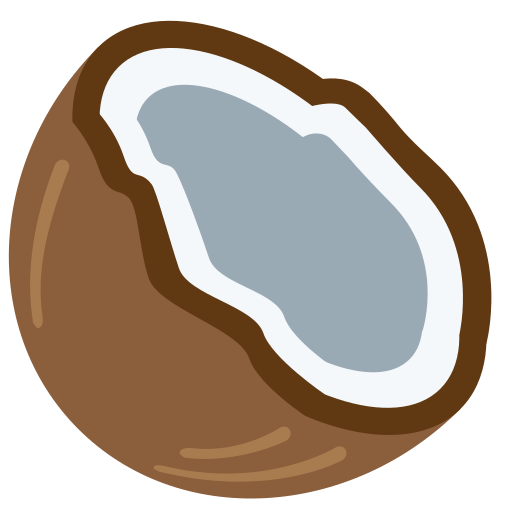
\includegraphics[height=4ex]{images/coconut.png}}
    \newcommand{\juice}{\includegraphics[height=4ex]{images/juice.png}}
    \newcommand{\heart}{
\includegraphics[height=4ex]{images/heart.png}}
    


%Formatting and Spacing
\setitemize[1]{noitemsep, parsep = 5pt, topsep = 5pt}
\setenumerate[1]{label = (\alph*), parsep = 1pt, topsep = 5pt}
\setlength\parindent{0pt}
\linespread{1.1}

% title
\title{\vspace{-1cm}CS 2051: Honors Discrete Mathematics \\Spring 2023 Homework 7 Supplement outline}
\author{Sarthak Mohanty, \tiny{Anant Gupta} }
\date{}

\begin{document}

\maketitle

% to do: fix titles
Title: ECC is the new RSA



\newtcolorbox{mybox}[2][]{enhanced,
before skip=2mm,after skip=2mm,
colback=black!5,colframe=black!50,boxrule=0.2mm,
attach boxed title to top left={xshift=1cm,yshift*=1mm-\tcboxedtitleheight},
varwidth boxed title*=-3cm,
boxed title style={frame code={
\path[fill=tcbcolback!50!black]
([yshift=-1mm,xshift=-1mm]frame.north west)
arc[start angle=0,end angle=180,radius=1mm]
([yshift=-1mm,xshift=1mm]frame.north east)
arc[start angle=180,end angle=0,radius=1mm];
\path[left color=tcbcolback!80!black,right color=tcbcolback!80!black,
middle color=tcbcolback!100!black]
([xshift=-2mm]frame.north west) -- ([xshift=2mm]frame.north east)
[rounded corners=1mm]-- ([xshift=1mm,yshift=-1mm]frame.north east)
-- (frame.south east) -- (frame.south west)
-- ([xshift=-1mm,yshift=-1mm]frame.north west)
[sharp corners]-- cycle;
},interior engine=empty,
},
fonttitle=\bfseries,
title={#2},#1}


\section*{Overview}

Over the past few weeks, we've covered number theory, as well as a nice application of it through the use of RSA cryptography.

\vspace{2mm}
Elliptic Curve Cryptography (ECC) is one of the most powerful cryptosystems in use today. Companies are using ECC everything to secure everything from our customers' HTTPS connections to how we pass data between our data centers. In fact, based on currently understood mathematics, ECC provides a significantly more secure foundation than first generation public key cryptography systems like RSA, for reasons we'll explore in detail later. The specific implementations you might learn in this supplement aren't as important as the general framework, understanding, and ideas you'll develop.

\vspace{2mm}
\textbf{Note.} As I was making this assignment, I stumbled across \href{https://andrea.corbellini.name/2015/05/17/elliptic-curve-cryptography-a-gentle-introduction/}{this} excellent blog post, and realized it covers some of these concepts a lot better than I ever could. For this reason, some of the exposition is adapted from this resource.


\section*{Cryptography Primer}
    Before we continue, it is beneficial to take a step back, and discuss cryptography as a whole. In this section, we discuss the difference between symmetric and asymmetric encryption, as well as what constitutes a ``hard" problem in cryptography. If you are already familiar, feel free to skip ahead.

\subsection*{Symmetric vs Asymmetric Systems}

    In cryptography, there are two main types of encryption algorithms: symmetric and asymmetric. 

    \vspace{3mm}
    \textbf{Symmetric, or private-key, encryption} uses the same key to both encrypt and decrypt the message. Symmetric encryption algorithms are generally faster and more efficient, but they require the sender and the recipient to share a secret key. The most prominent example is the AES cipher.\footnote{some of your classmates have chosen this as their group project!} 

    \vspace{3mm}
    On the other hand, \textbf{asymmetric, or public-key encryption} algorithms are slower and less efficient, but they allow the sender to send a message securely to the recipient without sharing a secret key. Examples include RSA, Diffie-Hellman, and ECCDH.

\subsection*{Trapdoor Functions}
    
    Trapdoor functions are an essential component of asymmetric encryption algorithms. A trapdoor function is a function that is easy to compute in one direction, but difficult to compute in the opposite direction without knowledge of additional information, such as a secret key.
    
    \vspace{2mm}
    As an example, the trapdoor function in RSA encryption is the modular exponentiation function, $c = m^e \mod N$, where $m$ is the plaintext, $e$ is the public exponent, $N$ is the modulus and $c$ is the ciphertext. The trapdoor information is the private key, which consists of the factors of $N$. In the opposite direction, decryption is performed by computing $m = c^d \mod N$, where $d$ is the private exponent derived from the private key.


\section*{Part 1: Diffie-Hellman (10 pts)}

\subsection*{Diffie-Hellman Key Exchange}

There is a classic analogy for the DH key exchange, which we present below: 

\begin{tcolorbox}[colback = CarnationPink!20]
    Professor Brito and Lianet (Brito’s wife!) have a famous Piña Colada recipe that they keep secret from the rest of the world. It is so secret in fact, that neither Brito nor Lianet know the full parts of the recipe! However, using their knowledge on how the Diffie-Hellman key exchange algorithm works, they have devised a unique way of making the drink.

    \vspace{2mm}
    To make their famous Piña Colada, Brito and Lianet have their own secret ingredients, which they mix separately. Brito mixes a secret amount of rum to a glass, while Lianet mixes a secret amount of pineapple juice to another glass. These individual mixtures represent the private keys of each party:

    $$\text{Brito:} \glass + \coconut + \rum = \mixedrum \quad \text{Lianet:} \glass + \coconut + \pineapple = \mixedpineapple$$
    
    \vspace{2mm}
    Next, they swap glasses. This represents the public key exchange. Note that because the ingredients were mixed in, it is very difficult for either Brito or Lianet to determine the exact contents of the current glass.

    $$\text{Brito: \mixedpineapple \quad Lianet: \mixedrum}$$
    
    Once they have exchanged their mixtures (or ``public keys"), they again use their own secret ingredients (or ``private keys") to mix with the others' drink to generate a shared ``secret key", in this case the final drink.

    $$\text{Brito:} \mixedpineapple + \rum = \pinacolada \quad \text{Lianet:} \mixedrum + \pineapple = \pinacolada$$

    \vspace{2mm}
     This shared secret key can be used to establish a secure communication channel, just like the delicious Piña Colada they created together.
     % $$\text{Brito}\quad\heart\quad\text{Lianet}$$
\end{tcolorbox}
    In this analogy, the rum and pineapple juice represent the private keys, while the remaining ingredients represent the public key exchange. The shared secret key is the final product, which can be used for secure communication between the two parties.


    \vspace{3mm}
    Let's now describe any algorithm that can transmit any information, not just piña coladas. The \textbf{Diffie-Hellman key exchange} is a cryptographic protocol that allows two parties to generate a shared secret key over an insecure communication channel. The protocol is named after its inventors, Whitfield Diffie and Martin Hellman, and is performed as follows:\footnote{taken verbatim from the CS 2051 Textbook.}
    \begin{enumerate}[label = \arabic*]
        \item Alice and Bob agree to use a prime $p$ and a primitive root $g$ of $p$.
        \item Alice chooses a secret integer $k_{1}$ and sends $g^{k_{1}} \pmod{p}$ to Bob.
        \item Bob chooses a secret integer $k_{2}$ and sends $g^{k_{2}} \pmod{p}$ to Alice.
        \item Alice computes $(g^{k_{2}})^{k_{1}} \pmod{p}$
        \item Bob computes $(g^{k_{1}})^{k_{2})}\pmod{p}$.
    \end{enumerate}

\subsection*{Trapdoor Function: Discrete Log Problem}
    The security of DH comes from the fact that an attacker, even given $g$, $p$, $g^{k_{1}} \pmod{p}$, and $g^{k_{2}} \pmod{p}$, \underline{cannot} efficiently calculate $g^{k_{1} k_{2}} \pmod{p}$. This leads us to a trapdoor function known as the \textit{discrete log problem}: $$\text{Given $g$, $p$, and $g^{x}\ \text{mod}\ p$, determine $x$}.$$ We will first demonstrate that we can break the discrete log problem if the parameters $x$ and $p$ are too small. Then, we will see through our implementations that as we increase the size of our numbers, the power of our attacks gets weaker. This cool fact is hopefully something you will see in your implementations.

    \begin{center}
        \textbf{Brute Force}
    \end{center}

    Recall that we want to find $a$ given $g$, $p$, and $g^{x}\ \text{mod}\ p$. The initial approach one might have would be to try all possible values of $x$. This takes $\mathcal{O}(p)$ time, which follows from the fact that $g$ is a generator.
    
    \begin{center}
        \textbf{Baby-Step Giant-Step algorithm}
        \footnote{this section was adapted from the blog post linked at the beginning of this supplement.}
    \end{center}

    Before we describe the algorithm, first note that any integer $x$ can be written as $x = am + b$, where $a$, $m$, and $b$ are arbitrary integers. For example, we can write $10 = 2 \cdot 3 + 4$. With this knowledge, we can rewrite the equation for the discrete log problem as follows:
    \begin{align*}
        g^{x} &\equiv y \pmod{p} \\
        g^{am + b} &\equiv y\pmod{p} \\
        g^{b} &\equiv y \cdot g^{-am} \pmod{p}
     \end{align*}

     The baby-step giant-step is a "meet in the middle" algorithm. In essence, instead of computing $g^{x} \pmod{p}$ for all values $x$, we instead calculate a few values for $g^{am} \pmod{p}$, as well as calculate a few values for $g^{am} \pmod{p}$. The algorithm works as follows:

     \begin{algorithm}
        \caption{\textsc{BabyStepGiantStep}}
        \label{alg:bsgs}
        \begin{algorithmic}
            \State $m = \lceil \sqrt{p}\ \rceil$
            \For{each $b$ in $0, \dots, m$}
                \State Store $g^{b}$ in a certain data structure (which one?)
            \EndFor
            \For{each $a$ in $0, \dots, m$}
                \State Calculate $y \cdot g^{-am}$.
                \State Check to see if there exists some $g^{b}$ such that $y \cdot g^{-am} = g^{b}$ (in $\mathcal{O}(1)$ time!)
            \EndFor
            \Return $x = am + b$
        \end{algorithmic}
    \end{algorithm}
    To understand why this algorithm works, forget the modulo for a second and take the equation $y = g^{am + b}$. Consider what follows:
    \begin{itemize}
        \item When $a = 0$ we are checking whether $y$ is equal to $g^{b}$, where $b$ is one of the integers from $0$ to $m$.
        \item When $a = 1$ we are checking whether $y$ is equal to $g^{m + b}$. We are comparing $y$ against all exponents from $m$ to $2m$.
        \item When $a = 2$ we are comparing $y$ against all exponents from $2m$ to $3m$.
        \item \dots
        \item When $a = m - 1$, we are comparing $y$ against all exponents from $(m - 1)m$ to $m^{2} = p$.
    \end{itemize}
    In other words, \textbf{we are checking all exponents from $0$ to $p$}. The time complexity of this algorithm is $\mathcal{O}(\sqrt{p})$.
    
    \begin{center}
    \textbf{General Number Field Sieve (GNFS)}
    \end{center}
    
    The General Number Field Sieve is a factorization algorithm that is particularly efficient for numbers with large prime factors. It is a multi-step process that involves finding a smooth polynomial and then finding the roots of that polynomial. GNFS is one of the most efficient known factorization algorithms for large integers.
    
    \vspace{3mm}
    We mention this attack not because of the implementation, but rather due to the implication. Algorithms such as GNFS get more efficient as the size of the numbers being factored get larger. The gap between the difficulty of factoring large numbers and multiplying large numbers is shrinking as the number (i.e. the key's bit length) gets larger. As the resources available to decrypt numbers increase, the size of the keys need to grow even faster. This is not a sustainable situation for mobile and low-powered devices that have limited computational power. The gap between factoring and multiplying is not sustainable in the long term.
    
    \vspace{2mm}
    All this means is that RSA is not the ideal system for the future of cryptography. In an ideal Trapdoor Function, the easy way and the hard way get harder at the same rate with respect to the size of the numbers in question. For this reason (and a few others discussed later), we need a better public key system. In 1985, such a system was found, revolving around an (then) arcane field known as elliptic curves.

    \begin{tcolorbox}[enhanced,interior style={top color=Plum!20,bottom color=Plum!30}]
        In this part, you'll implement the Actor class, which contains methods to emulate the Diffie-Hellman key exchange:
    
    % mix with black
        \begin{mybox}[
            colframe=Cerulean!50!black,
            colback=Cerulean!30,
            colbacktitle=Cerulean!,
            % fonttitle=\bfseries,
            coltitle=Cerulean!30!black
            ]{Actor}
            A given actor has access to the public parameters $p$ and $g$, as well as its own private key $k$.
            \begin{itemize}
                \item \lstinline{computePublicKey(self)}: Computes and returns the public key.
                \item \lstinline{computeSecret(self, offer)}: Takes in a public key and assigns to the actor the corresponding shared secret.
            \end{itemize}
    
        \end{mybox}
    
        You'll then try to break this key exchange by implementing the BadActor class, containing the following methods:
    
        \begin{mybox}[
            colframe=purple!50!black,
            colback=purple!40,
            colbacktitle=purple!50!white,
            % fonttitle=\bfseries,
            coltitle=purple!30!black,
            ]{BadActor}
            The bad actor has access to the same public parameters as above, but \underline{not} the private key.
            \begin{itemize}
                \item \lstinline{brute(self, y)}: This function solves the discrete log problem using brute force.
                \item \lstinline{bsgs(self, y)}: This function solves the discrete log problem using the baby-step giant-step algorithm.
                \item \lstinline{stealSecret(self, actor1, actor2, attack)}: This method will use the attacks outlined above to intercept the Actors' shared secret.
            \end{itemize}
        \end{mybox}
    
        \vspace{2mm}

        To-do: Rewrite this, talk about built in pow method

        % https://github.com/python/cpython/blob/109fc2792a490ee5cd8a423e17d415fbdedec5c8/Objects/longobject.c#L4244-L4447

        Tip: Calculating $g^{a}$ directly and then finding its remainder when divided by $p$ is impractical and will not work with large numbers. This is because $g^{a}$ will be a huge number for large $g, a$. Instead, you should use an algorithm that employs the binary expansion of the exponent $a$. The details of this algorithm can be found in Section 4.2 of the textbook, under ``Modular Expoonentiation".
    \end{tcolorbox}



\section*{Part 2: Enter Elliptic Curves (8 pts)}

The standard form for an elliptic curve is $$y^{2} = x^{3} + ax + b,$$ where $a$ and $b$ are constants. This is referred to as the Weierstrass equation for an elliptic curve. For reasons that will be discussed later, also include the point $\{\infty\}$ in this function.

\subsection*{The Group Law}
    One important aspect of elliptic curves is that we can start with two points, or even one point on an elliptic curve, and produce another point. To do this, start with two points $P = (x_{1}, y_{1})$, $Q = (x_{2}, y_{2})$ on an elliptic curve $E$. Now draw a line $L$ through $P$ and $Q$. This line will intersect $E$ at a third point $R'$. (such a point always exists, and you'll prove it when trying to calculate the exact value of this point below!) Finally, reflect $R'$ across the $x$-axis to obtain $R$. We define $$P + Q = R.$$ You can see an example of this addition in Figure (\ref{fig:point_addition}).

\begin{figure}[htbp]
    \centering
    
    \begin{subfigure}[t]{.45\textwidth}
        \centering
        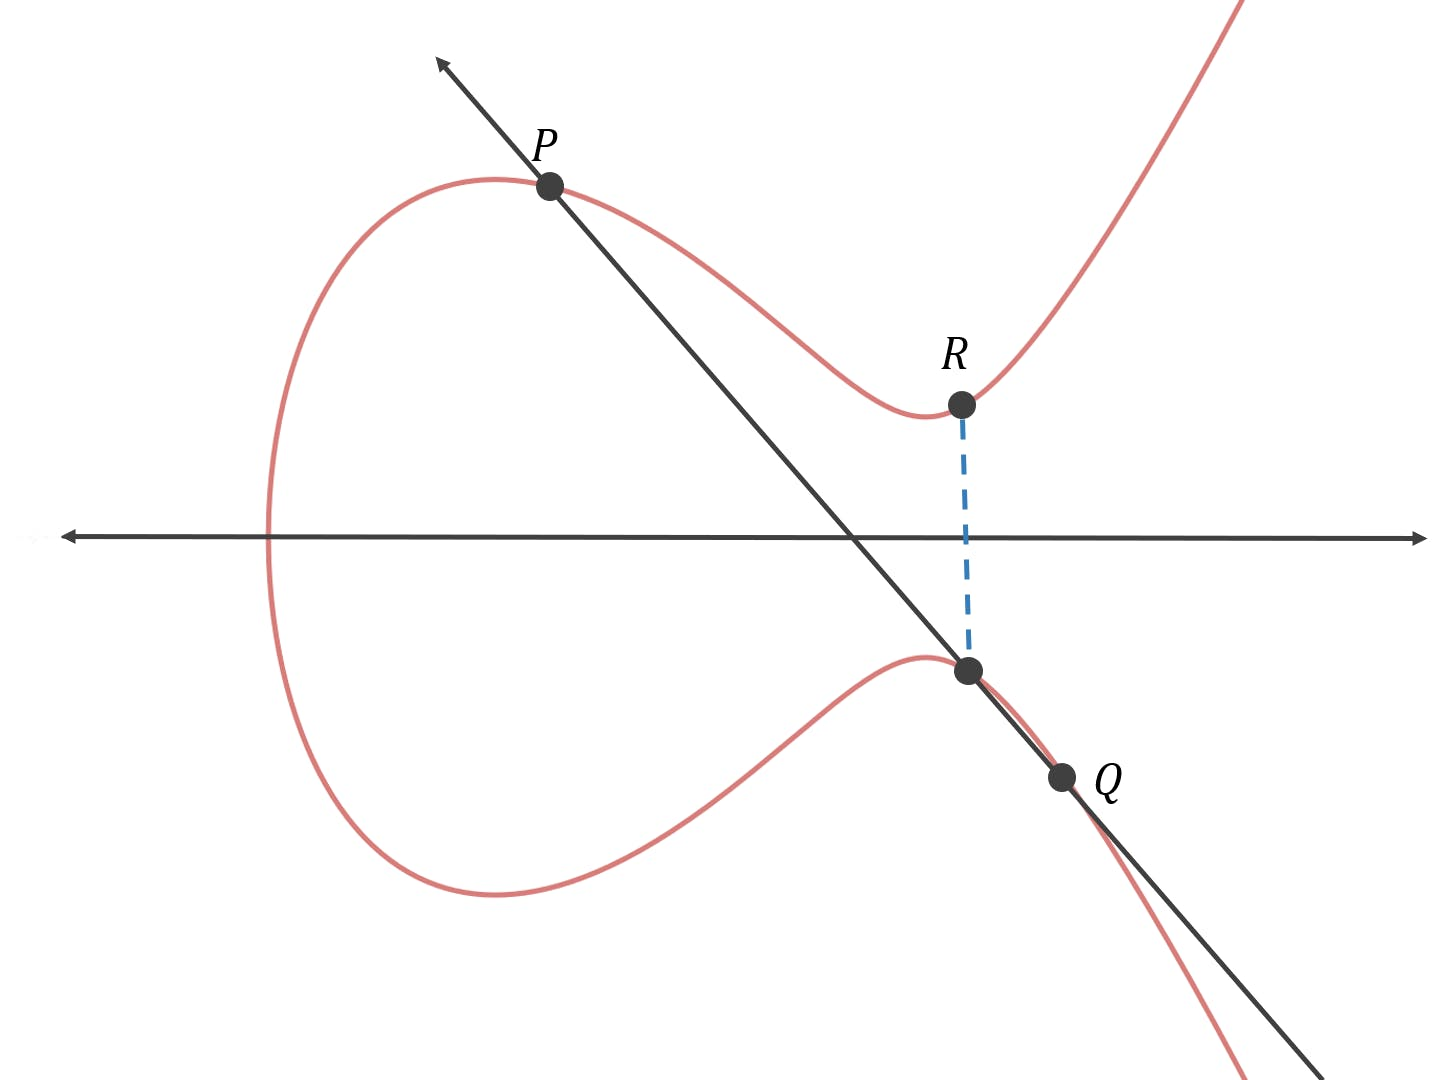
\includegraphics[scale = 0.15]{images/point_addition.jpeg}
        \caption{Point Addition}
        \label{fig:point_addition}
    \end{subfigure}
    \begin{subfigure}[t]{.45\textwidth}
        \centering
        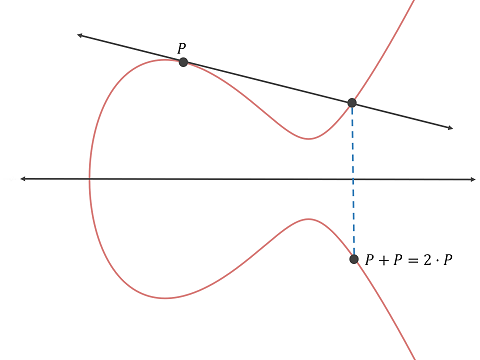
\includegraphics[scale = 0.8]{images/point_scalar_multiplication.png}
        \caption{Point scalar multiplication}
        \label{fig:point_multiplication}
    \end{subfigure}
    \caption{Group law visualized.}
    \label{fig:edge_case}
\end{figure}


\begin{tcolorbox}[enhanced,interior style={top color=Plum!20,bottom color=Plum!30}]
    \textbf{In this part, you'll implement the following functions:}
    \begin{itemize}
        \item \lstinline{point_addition(elliptic_curve, P, Q)}: This function takes in an elliptic curve 
        \item \lstinline{point_scalar_multiplication(elliptic_curve, k, P))}: This function takes in an elliptic curve of the form described, a scalar integer $k$, and a point $P$, and repeatedly multiplies this result to output a number.
    \end{itemize}
    You can run \lstinline{visualize_addition} and \lstinline{visualize_multiplication} to generate the corresponding visualizations mentioned above. If you want more examples, there's an interactive tool \href{https://andrea.corbellini.name/ecc/interactive/reals-add.html}{here}
    Notes: This part is just algebra and geometry. Since I know it's been a while since many of you touched this, here's a few steps you get you started.
    \begin{itemize}
        \item For point addition, we assumed that $P \ne Q \ne \infty$. For this reason, we can draw the line $L$ through $P_{1}$ and $P_{2}$. Its slope is $$m = \frac{y_{2} - y_{1}}{x_{2} - x_{1}}.$$ If $x_{1} = x_{2}$, then $L$ is vertical, so the resulting point is just $\infty$. Now let's assume that $x_{1} \ne x_{2}$. The equation of $L$ is then $$y = m(x - x_{1}) + y_{1}.$$ To find the intersection of this line with the elliptic curve, we can substitute the above equation into the formula for an elliptic curve $$y^{2} = x^{3} + ax + b.$$ Finally, we can reflect the above point across the $x$-axis to obtain the point $P_{3} = (x_{3}, y_{3})$.
        \item For point scalar multiplication, we have that $P = Q = (x_{1}, y_{1})$. When two points on a curve are very close to each other, the line through them approximates a tangent line. Therefore, when the two points coincide, we take the line $L$ through them to be the tangent tine. Implicit differentiation allows us to find the slope $m$ of $L$: $$2y \frac{dy}{dx} = 3x^{2} + a,\text{\quad so\quad} m = \frac{dy}{dx} = \frac{3x_{1}^{2} + a}{2y_{1}}.$$ If $y_{1} = 0$ then the line is vertical and we set $P_{1} + P_{2} = \infty$, as before. Otherwise, we plug in values into $L$ and solve as before.
    \end{itemize}
    
\end{tcolorbox}

\section*{Part 3: In The Field (12 pts)}
    The elliptic curve cryptography (ECC) uses elliptic curves taken over the finite field $\mathbb{F}_{p}$ (where $p$ is prime and $p > 3$). For example, the ``Bitcoin curve" secp256k1 takes the form: $$y^{2} \equiv x^{3} + 7 \pmod{p}.$$ Firstly, what do these curves look like? Well, they actually look pretty random. For example, the bitcoin curve mapped over mod $3$ looks like

    \begin{figure}[htbp]
        \centering
        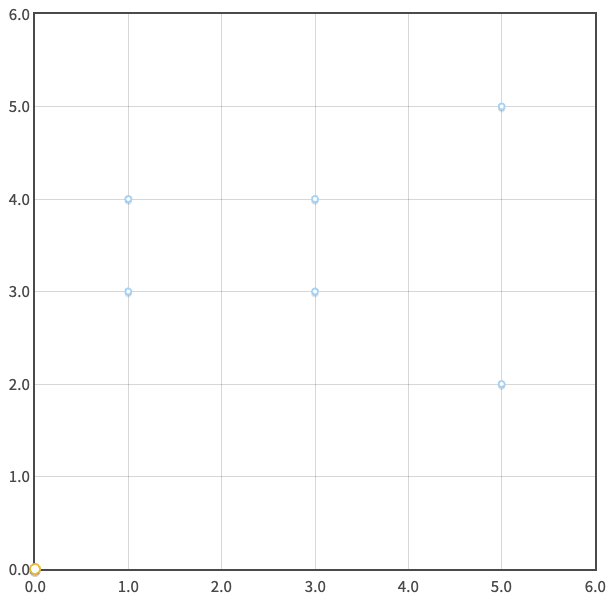
\includegraphics[scale = 0.4]{images/generate_points.png}
        \caption{An elliptic curve over a Galois field.}
        \label{fig:generate_points}
    \end{figure}

    The group law over $\mathbb{F}_{p}$ is similar, but not identical to in the field of real numbers. It is stated (and proven) in \href{https://arxiv.org/pdf/1710.00214.pdf}{this} research paper.

    \begin{tcolorbox}[enhanced,interior style={top color=Plum!20,bottom color=Plum!30}]
        In this part, you'll visualize elliptic curves over finite fields, as well as implement point addition and point multiplication over these fields
    
        \textbf{In this part, you'll implement the following functions:}
        \begin{itemize}
            \item \lstinline{generate_point_cloud(a, b, p)}: This takes in an elliptic curve and returns a set of all valid points in the curve over that field.
            \item \lstinline{point_addition(P, Q, a, b, p)}: This function takes in an elliptic curve and two points, and adds them.
            \item \lstinline{point_scalar_multiplication(P, n, a, b, p)}: This function takes in an elliptic curve of the form described, a scalar integer $k$, and a point $P$.
        \end{itemize}
        After completing each function, you should be able to run \lstinline{visualize_curve}, \lstinline{visualize_point_addition}, and \lstinline{visualize_point_scalar_multiplication} to check your work.
    \end{tcolorbox}

\section*{Part 4: ECC in Action: Elliptic-curve Diffie Hellman (10 pts)}

% You've devleoped some undrestanding of how elliptic curves work, but it's naturarl to doubt the connection between them. This is where yopu're wrong. Note that... this is called \textit{order independence}. This makes it really easy to modify diffie hellman to accomodate our elliptic curves, as follows:

% This order independence also makes it easy to see why ECC takes less storage space than Diffie-Hellman, 

\subsection*{The Elliptic-curve Discrete Log Function}



    \vspace{3mm}
    Trapdoor function in Elliptic Curve Cryptography (ECC). In ECC, the trapdoor function is the scalar multiplication operation $Q = kP$, where $P$ is a point on the elliptic curve, $k$ is the scalar and $Q$ is the result of the scalar multiplication. The trapdoor information is the private key, which is the scalar $k$. Decryption is performed by computing $Q = -kP$.


For carefully chosen (by cryptographers) finite fields and elliptic curves, the ECDLP problem has no efficient solution.

The multiplication of elliptic curve points in the group $\mathbb{F}_{p}$ is similar to exponentiation of integers in the group $\mathbb{Z}_{p}$ (this is known as multiplicative notation) and this is how the ECDLP problem is similar to the DLP problem (discrete logarithm problem).

See \href{https://www.youtube.com/watch?v=gAtBM06xwaw}{this} video for implementation details


% \begin{tcolorbox}[enhanced,interior style={top color=Plum!20,bottom color=Plum!30}]
    

% % mix with black
%     \begin{tcolorbox}[title=Actor Class,
%         colframe=Cerulean!50!black,
%         colback=Cerulean!50,
%         arc=1mm,colbacktitle=Cerulean!50!white,
%         fonttitle=\bfseries,coltitle=Cerulean!50!black,
%         % attach boxed title to top center=
%         % {yshift=-2mm,yshifttext=-1mm},
%         % boxed title style={
%         % interior style={fill=none,
%         % top color=green!30!white,
%         % bottom color=green!20!white}}
%         ]
%         \begin{itemize}
%             \item \lstinline{computePublicKey(self)}: See docs for details
%             \item \lstinline{computeSecret(self, offer)}: See docs for details
%         \end{itemize}
%     \end{tcolorbox}

%     \begin{tcolorbox}[title=Actor Class,
%         colframe=purple!50!black,
%         colback=purple!50,
%         arc=1mm,colbacktitle=purple!50!white,
%         fonttitle=\bfseries,coltitle=purple!50!black,]
%     \begin{itemize}
%         \item \lstinline{brute(self, g, y, n):}: This function takes in the parameters for the discrete log problem, and returns the correct answer using brute force.
%         \item \lstinline{bsgs(self, g, y, p)}: Same thing as above, but with baby-step giant-step algorithm.
%     \end{itemize}
%     \end{tcolorbox}
% \end{tcolorbox}

\begin{tcolorbox}[enhanced,interior style={top color=Plum!20,bottom color=Plum!30}]
    Finally, the part you've been waiting for. In this part, you'll implement an Elliptic-Curve Diffie Hellman key change algorithm. The functions you will implement are similar to those in Part 1. First, you'll implement the Actor class:

    % mix with black
    \begin{mybox}[
        colframe=Cerulean!50!black,
        colback=Cerulean!30,
        colbacktitle=Cerulean!,
        % fonttitle=\bfseries,
        coltitle=Cerulean!30!black
        ]{Actor}
        A given actor has access to the public curve parameters $(a, b, n)$, the public generator point $P$, and a private key $k$.
        \begin{itemize}
            \item \lstinline{computePublicKey(self)}: Computes and returns the public key.
            \item \lstinline{computeSecret(self, offer)}: Takes in a public key and assigns to the actor the corresponding shared secret.
        \end{itemize}

    \end{mybox}

    You'll then try to break this key exchange by implementing the BadActor class, containing the following methods:

    \begin{mybox}[
        colframe=purple!50!black,
        colback=purple!40,
        colbacktitle=purple!50!white,
        % fonttitle=\bfseries,
        coltitle=purple!30!black,
        ]{BadActor}
        The bad actor has access to the same public parameters as above, but \underline{not} the private key.
        \begin{itemize}
            \item \lstinline{brute(self, Q)}: This function solves the ECDLP using brute force.
            \item \lstinline{bsgs(self, Q)}: This function solves the ECDLP using the baby-step giant-step algorithm.
            \item \lstinline{stealSecret(self, actor1, actor2, attack)}: This method will use the attacks outlined above to intercept the Actors' shared secret.
        \end{itemize}
    \end{mybox}
\end{tcolorbox}


% https://arstechnica.com/information-technology/2015/11/op-ed-how-did-they-break-diffie-hellman/?comments=1&comments-page=1#comment-30128933

\subsection*{Conclusion}

    \subsubsection*{RSA vs ECC}

    Since RSA and ECC essentially serve the same purpose, there have been many heated discussions as to which implentation to use. The main pro of using ECC is the fact that it uses fewer memory and CPU resources, important as mobile computing becomes more ubiquitous. However, there are a few flaws with ECC. First, there are only a few curves that work and the NIST is in contorl of most of them, but people distrust NIST. Second, 

    \vspace{2mm}
    Finally, neither ECC nor RSA are secure against quantum computers. 



    \subsubsection*{Real World Application}

    Even with all those downsides, more and more companies are using ECC, including

    \begin{center}
        Amazon, Bing, Dropbox, Facebook, Flickr, GitHub, Instagram, \\
        LinkedIn, MSN, Netflix, Pinterest, PirateBay, Quora, Snapchat, \\
        SoundCloud, Spotify, StackOverflow, Tumblr, Twitter, Uber, \\
        Vimeo, Vine, Yahoo, Yelp, YouTube, Wikipedia, Wordpress,\dots
    \end{center}

Two prominent examples:
    \begin{itemize}
        \item \href{https://chat.openai.com/chat}{ChatGPT}
        \item \href{https://proton.me/blog/elliptic-curve-cryptography}{ProtonVPN}
    \end{itemize}

    to do: explain how you can see ecc implentation on website. Click on lock on top left of website, click on ``connection is secure", click on ``certificate is valid", you should see ECC used for certificate

    
    assymetric not often used since takes long time. Instead, key exchange is done using assymetric andthen symmetric is used to send the actual messages, as can be seen \href{https://github.com/nakov/Practical-Cryptography-for-Developers-Book/blob/master/asymmetric-key-ciphers/ecc-encryption-decryption.md}{here}


\section*{Submission Instructions (10 pts)}
    After you fill the appropriate functions, submit the following files to Gradescope and make sure you pass all test cases:
    \begin{itemize}
        \item \lstinline{diffie_hellman.py}
        \item \lstinline{elliptic_curves.py}
        \item \lstinline{ECDH.py}
    \end{itemize}

    \vspace{3mm}
    \textbf{Notes}
    \begin{itemize}
        \item The autograder may not reflect your final grade on the assignment. We reserve the right to run additional tests during grading.
        \item Do not import additional packages, as your submission may not pass the test cases or manual review.
    \end{itemize}

    
    % These factoring algorithms get more efficient as the size of the numbers being factored get larger. The gap between the difficulty of factoring large numbers and multiplying large numbers is shrinking as the number (i.e. the key's bit length) gets larger. As the resources available to decrypt numbers increase, the size of the keys need to grow even faster. This is not a sustainable situation for mobile and low-powered devices that have limited computational power. The gap between factoring and multiplying is not sustainable in the long term.

\section*{References}

\begin{itemize}
    \item explanation for group law name is \href{https://www.math.brown.edu/reschwar/M1540B/elliptic.pdf}{here}
    \item why infinity is added \href{https://crypto.stackexchange.com/questions/70507/in-elliptic-curve-what-does-the-point-at-infinity-look-like}{here}
    \item This (heavy) textbook is a good resource if you want to explore the mathematics of elliptic curves in further detail.
    \item Again, the amazing blog post mentioned above.
\end{itemize}
% \begin{mybox}[colbacktitle=green]{My title}
% \lipsum[2]
% \end{mybox}
% \begin{mybox}[colbacktitle=red]{My title}
% \lipsum[3]
% \end{mybox}

\end{document}